\section{NVIDIA GPU 架构历史}

大家好，在本文章中我将带大家了解NVIDIA推出的各种GPU架构。我们先从这张展示的图像开始，该图像表明自1998年以来
，NVIDIA已推出了众多架构。我们将从NVIDIA于2010年推向市场的Fermi架构开始探索。不过，我们将跳过一些早
期架构，因为它们已不再使用。

\begin{figure}
    \centering
    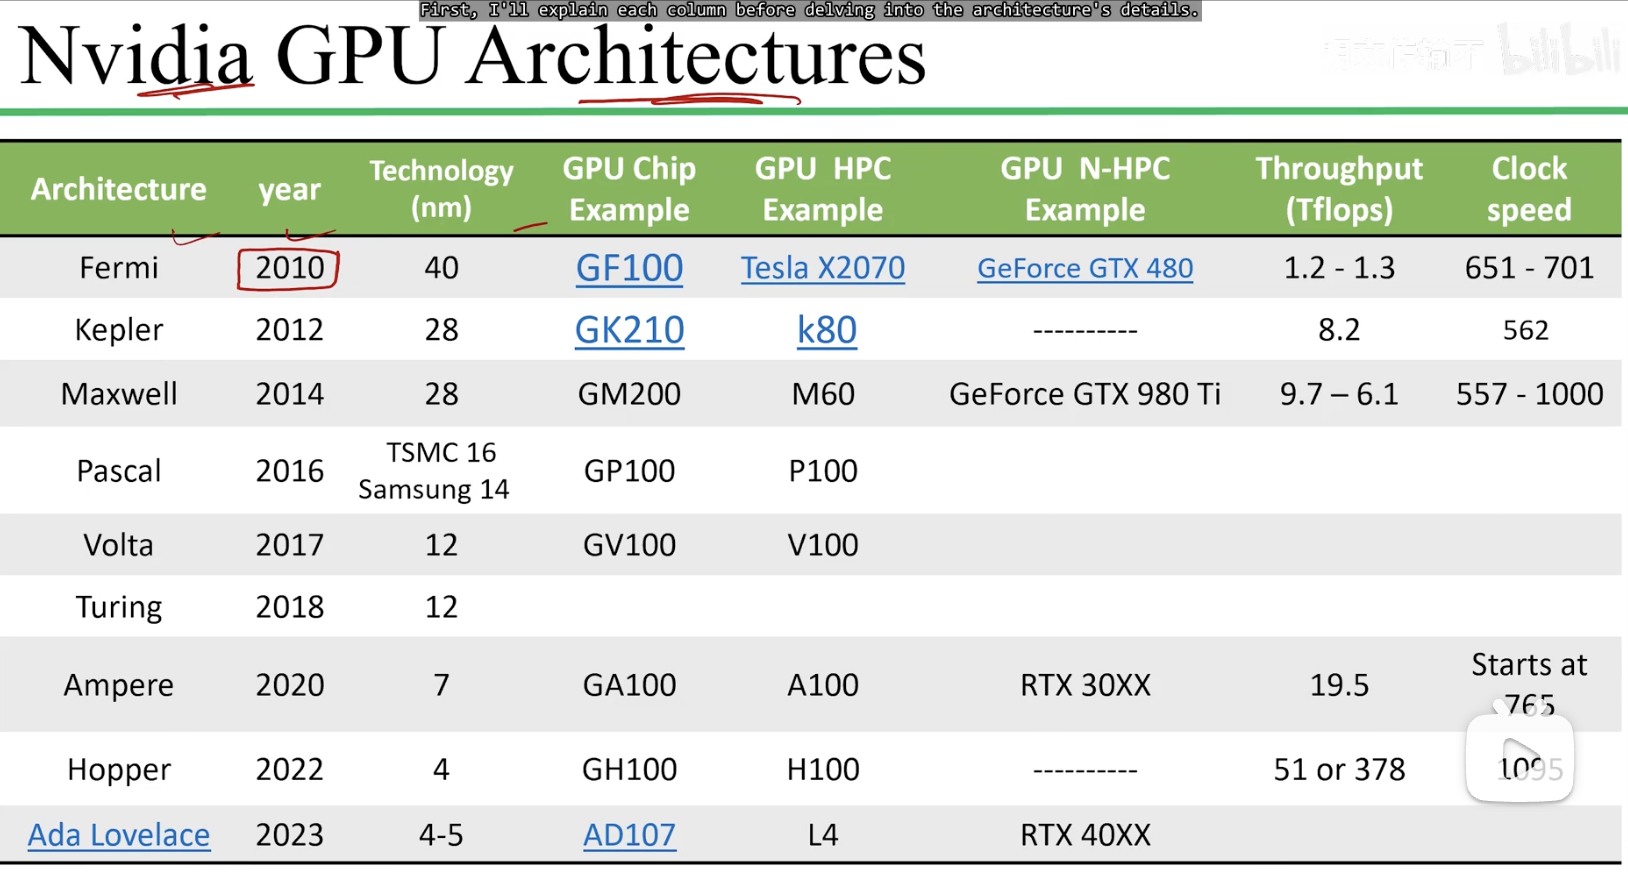
\includegraphics[width=0.75\linewidth]{resources/cuda-022.png}
    \caption{GPU 架构历史}
    \label{fig:placeholder}
\end{figure}


这张展示的表格列出了NVIDIA自2010年以来推出的所有架构。首先，在深入讲解各架构细节之前，我会先解释每一列的含义。
第一列显示了NVIDIA引入的架构名称，第二列显示了他们各自的发布时间。接下来是GPU芯片示例列，该列提供了每个架构的代
表性电子芯片。在后续讲解中，我会为每个架构突出展示两款不同的GPU型号，它们被分为两列，第一列是HPC GPU，即高性能计
算GPU。第二列是非高性能计算GPU，即面向普通用户或普通消费者的GPU。最后，我们还有两列专门用于评估各架构的计算能力
或性能指标。

在本表中，我仅选取了两个关键参数进行比较。第一个是吞吐量，用于计算每秒浮点运算次数。第二个是时钟频率。对于这些参数，在大
多数情况下，我会为高性能计算GPU显示一个数值，为面向普通消费者的GPU显示另一个数值。

\subsection{Fermi架构}

我将深入讲解NVIDIA GPU的各种架构。我们从 Fermi架构开始。Fermi架构由NVIDIA于2010年推出，是
GPU设计与技术的一次重大飞跃。

基于Fermi的GPU采用40纳米工艺制造。一个基于Fermi架构的GPU芯片示例是GF100芯片，该芯片被用于生产多种
GPU，既用于高性能计算，也用于普通用户或普通消费者。另一方面，GeForce GTX 480则专为普通消费者和游戏玩家设计
。例如其中一款高性能计算GPU是基于该芯片或该架构的Tesla X2070。如果你关注这些数字，这些性能指标数字，你可能会
疑惑，为什么专为普通用户设计的GTX480在性能上似乎优于Tesla X2070？在性能指标方面，这两款GPU的吞吐量分别
可达1.2和1.3万亿次浮点运算，每秒TFlops时钟频率分别为655和701 Mhz。例如，GTX 480的时钟频率为
700，而 X2070 GPU仅为651。

\begin{figure}
    \centering
    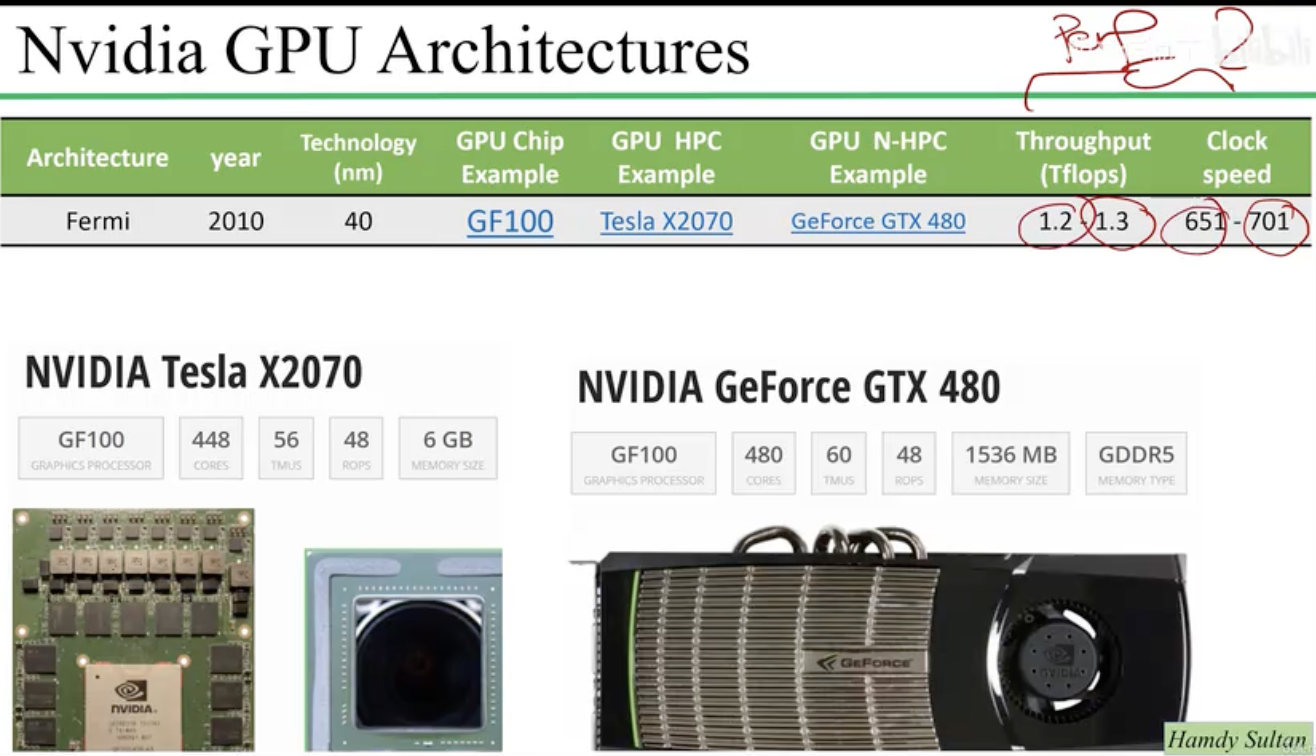
\includegraphics[width=0.75\linewidth]{resources/cuda-023.png}
    \caption{Fermi 架构示例}
    \label{fig:placeholder}
\end{figure}


要解答这一点，必须理解，评估GPU性能并非一目了然。GPU的整体性能受多种因素和指标影响，而不仅仅是这两个指标。仅凭TFlops或时钟频率这样的单一指标不足以全面衡量GPU的整体能力。此外，某一指标看似有意，在另一背景下可能并非如此。例如，

更高的时钟频率虽然能加速任务，但也可能导致功耗和能耗增加，这对某些系统来说可能并不理想。

另外需要澄清的是，GTX GPU看似优于X2070 GPU的TFlops值或吞吐量值，仅针对单精度运算。这并非针对GPU
中所有核心的整体性能。我们通过一个例子深入说明这一点。当我们打开Tech Power UP网站查看这两款GPU时，你会注意
到X2070 GPU的双精度性能，如此处所示约为 582.8 GFLOPS，该数值高于GTX GPU的数值。这表明在双精度
任务方面，X2070 GPU的性能几乎是GTX GPU的四倍。GTX 480 GPU仅有168.1 GFLOPS，这类任务之一
就是科学仿真。然而在纹理和像素填充率等指标上，这些指标需要单精度运算。GTX480 GPU则优于 X2070 GPU，这也
符合其面向图形游戏和日常应用的定位。

\subsection{Kepler架构}

让我们回到幻灯片讲解下一个架构Kepler。在Fermi发布两年后，NVIDIA推出了Kepler架构。观察这一列可以明
显看出NVIDIA大致每一年或两年就会发布一款新架构。Kepler架构采用28纳米工艺制造，而Fermi架构使用的是40
纳米工艺。

NVIDIA的 GK210芯片主要应用于Tesla K80 GPU而闻名，该GPU是一款高性能计算GPU卡。令人意外的是，
Tesla K80 GPU包含两颗芯片，而非一颗在一块板卡上使用了两颗GK210芯片。凭借单板上集成的两颗芯片，K80GPU实现了约8.2万亿次浮点运算每秒的吞吐量。
这相比Fermi架构提升了六倍。但需要注意的是，该吞吐量值包含了两颗芯片的
总和，这意味着每颗芯片及每颗GK210芯片大约提供4.1万亿次浮点运算每秒。除了K80GPU，基于该芯片的其他广为人知的
GPU并不多，大多数面向消费市场的其他Kepler GPU均基于不同的芯片。

\begin{figure}
    \centering
    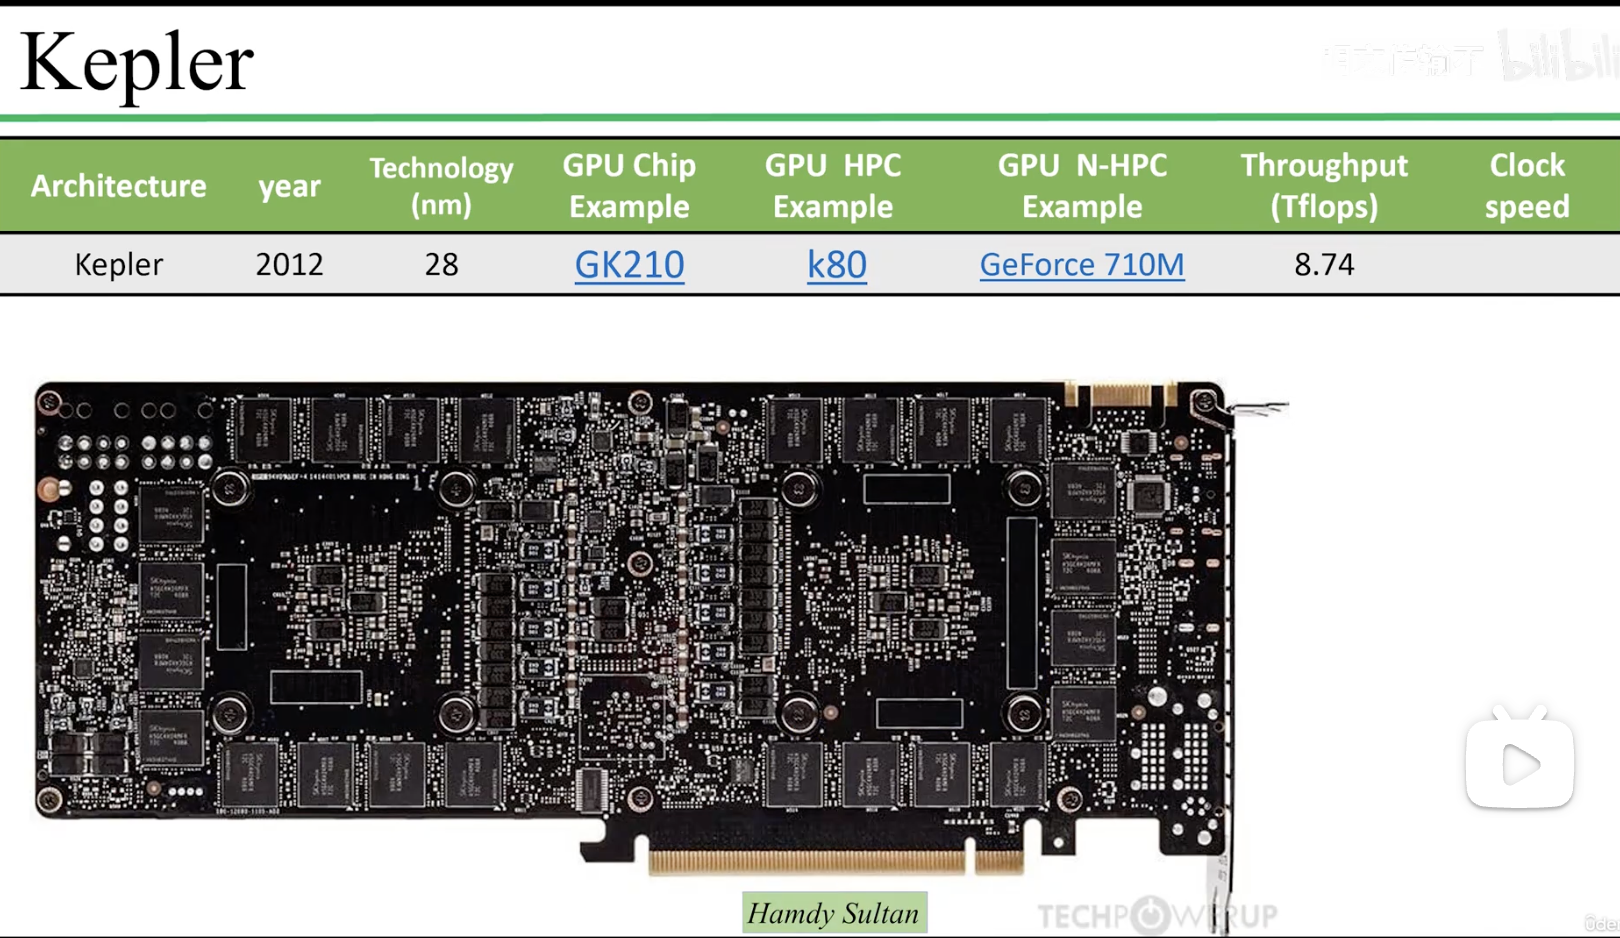
\includegraphics[width=0.75\linewidth]{resources/cuda-024.png}
    \caption{Kepler 架构}
    \label{fig:placeholder}
\end{figure}


关于Kepler，我还想提一下它的升级版本。如需查看基于各类Fermi芯片的更完整GPU列表，
可参考Tech Power UP网站的Fermi专区，有时NVIDIA会发布同一架构的升级版或增强版。例如，Kepler最初由NVIDIA于2012
年推出，但在2013年至2015年间出现了更更新的Kepler版本。如此图所示，你可以看到Maxwell架构也发生了类似
情况，当你在Tech Power APP网站上查看GK210芯片时会发现其发布时间为2014年，与表格中提供的2012年不
同，表格中的发布日期指的是该架构的最初版本。

\subsection{Maxwell架构}

Maxwell架构由NVIDIA于2014年推出，是GPU领域的一项重大进步，它同样采用28纳米工艺制造，该架构的旗舰芯
片之一是GM200，该芯片被用于Tesla M60 GPU，专为高性能计算设计。此外，对于游戏玩家而言，GeForce GTX980 Ti
是另一款基于Maxwell架构的GPU。在吞吐量方面，M60 达到9.7万亿次浮点运算每秒，而GTX GPU
为6.1万亿次浮点运算每秒。在时钟频率方面，M60运行于557兆赫，而GTX则达到1000兆赫。再说一遍，这款专用于高性
能计算的M60时钟频率较低，这直接关联到能耗问题。

\subsection{Pascal架构}

从Pascal架构开始，高性能计算GPU卡采用了字母加100的命名模式。在Pascal架构中，GPU名称为P100，其中
P代表Pascal，这一趋势延续到Volta、Ampere和Hopper架构，它们分别被命名为V100、A100和H100。这种命
名方式也体现在GPU芯片上，如我们所见，Pascal架构中有GP100，随后在Volta、Ampere和Hopper中分别有GV100、GA100和GH100。Pascal架构于2016年推出，采用16纳米和14纳米工艺制造。你可
能会疑惑，为何同一架构会采用两种不同的工艺？主要原因在于当时市场上不同制造商可获得的技术水平不同。有些厂商能使用更先进的
14纳米工艺生产GPU，而其他公司仍在使用16纳米工艺。尽管存在这些差异，各公司仍能基于相同的Pascal架构生产GPU
，只是纳米尺寸不同。

关于Pascal架构，我不会在此过多展开，因为我会在后续文章中结合白皮书或数据手册详细讲解剩余架构。这里只提一点，如我们
所见，性能提升极为显著。只需看看Hopper架构的吞吐量，并将其与Fermi的数值进行比较，一切便一目了然。从Fermi
架构的1.2万亿次浮点运算每秒，到如今Hopper架构的378万亿次浮点运算每秒，我此处略过所写的51万亿次浮点运算每秒
，因为它将在Hopper架构文章中深入解释。
